\documentclass[a4paper]{article}
%\usepackage[singlespacing]{setspace}
\usepackage[onehalfspacing]{setspace}
%\usepackage[doublespacing]{setspace}
\usepackage{geometry} % Required for adjusting page dimensions and margins
\usepackage{amsmath,amsfonts,stmaryrd,amssymb,mathtools,dsfont} % Math packages
\usepackage{tabularx}
\usepackage{colortbl}
\usepackage{listings}
\usepackage{amsmath}
\usepackage{amssymb}
\usepackage{enumerate}
\usepackage{enumitem}
\usepackage{amsthm}
\usepackage{subcaption}
\usepackage{float}
\usepackage[table,xcdraw]{xcolor}
\usepackage{tikz-qtree}
\usepackage{tikz}
\usepackage{forest}
\usepackage{changepage,titlesec,fancyhdr} % For styling Header and Titles
\pagestyle{fancy}
\renewcommand{\headrulewidth}{0.5pt} % Linienbreite anpassen, falls gewünscht
\renewcommand{\headrule}{
    \makebox[\textwidth]{\rule{1.0\textwidth}{0.5pt}} 
}
\usepackage{amsmath}
\pagestyle{fancy}
\usepackage{diagbox}
\usepackage{xfrac}

\usepackage{pgfplots}
\usepackage{pgfplotstable}
\pgfplotsset{compat=1.18}

\usepackage{enumerate} % Custom item numbers for enumerations

\usepackage[ruled]{algorithm2e} % Algorithms

\usepackage[framemethod=tikz]{mdframed} % Allows defining custom boxed/framed environments

\usepackage{listings} % File listings, with syntax highlighting
\lstset{
	basicstyle=\ttfamily, % Typeset listings in monospace font
}

\usepackage[ddmmyyyy]{datetime}


\geometry{
	paper=a4paper, % Paper size, change to letterpaper for US letter size
	top=3cm, % Top margin
	bottom=3cm, % Bottom margin
	left=2.5cm, % Left margin
	right=2.5cm, % Right margin
	headheight=25pt, % Header height
	footskip=1.5cm, % Space from the bottom margin to the baseline of the footer
	headsep=1cm, % Space from the top margin to the baseline of the header
	%showframe, % Uncomment to show how the type block is set on the page
}
\lhead{\vspace{0.5\baselineskip}Übungsblatt 6}
\chead{\bfseries{Einführung in Verteilte Systeme\\Sommersemester 2025}}
\rhead{\vspace{0.5\baselineskip}Werner, 7987847}
\fancyheadoffset[R]{0cm}

\begin{document}
\setcounter{section}{6}
\subsection{Spanning Tree}
Gegeben sei die in der Abbildung gezeigte Topologie von Netzwerken (b-f) und Switches (S3-S76).\\\\
Alle eingezeichneten Switches nutzen das Spanning-Tree Protokoll, um Weiterleitungsschleifen zu verhindern. Switch-IDs entsprechen den Bezeichnungen der Switches (“S76” hat ID=76). Die Pfadkosten sind für alle Ports gleich.\\\\
Bestimmen und zeichnen Sie den resultierenden Spanning-Tree, indem Sie:\\
1) das Root-Switch bestimmen und markieren,\\
2) für jedes Switch den Abstand zum Root-Switch angeben (die Abstände beginnen mit 1)\\
3) für jedes Switch die blockierten Ports durchstreichen.\\

\begin{center}
    \scalebox{1.75}{
        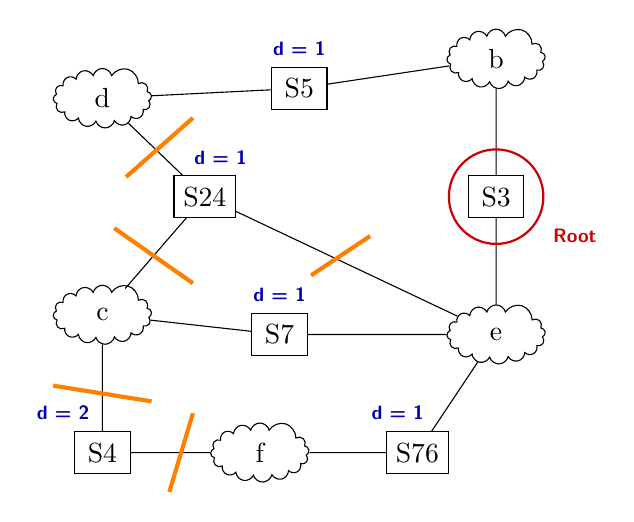
\begin{tikzpicture}[
          cloudnode/.style={draw, cloud, cloud puffs=15.7, minimum width=1.25cm, minimum height=0.75cm, align=center, cloud ignores aspect},
          switchnode/.style={draw, rectangle, minimum width=2em, minimum height=1.5em},
          node distance=2cm
        ]
        
        % Nodes
        \node[cloudnode] (b) at (5,3.5) {b};
        \node[cloudnode] (c) at (0,0.25) {c};
        \node[cloudnode] (d) at (0,3.0) {d};
        \node[cloudnode] (e) at (5,0) {e};
        \node[cloudnode] (f) at (2,-1.5) {f};
        
        \node[switchnode] (S3) at (5,1.75) {S3};
        \node[switchnode] (S4) at (0,-1.5) {S4};
        \node[switchnode] (S5) at (2.5,3.125) {S5};
        \node[switchnode] (S7) at (2.25,0) {S7};
        \node[switchnode] (S24) at (1.3,1.75) {S24};
        \node[switchnode] (S76) at (4,-1.5) {S76};
        
        % Edges
        \draw (b) -- (S3) -- (e);
        \draw (b) -- (S5) -- (d);
        \draw (d) -- (S24) -- (c);
        \draw (S24) -- (e);
        \draw (c) -- (S7) -- (e);
        \draw (c) -- (S4) -- (f);
        \draw (e) -- (S76) -- (f);

        \definecolor{darkred}{rgb}{0.8, 0.0, 0.0};

        \draw[darkred, thick] (S3) circle [radius=0.6cm];
        \node[darkred] at (6, 1.25) {\sffamily\scriptsize \textbf{Root}};

        \definecolor{darkblue}{rgb}{0.0, 0.0, 0.7}; % dark navy blue

        \node[darkblue] at (-0.5, -1) {\sffamily\scriptsize \textbf{d = 2}}; % S4
        \node[darkblue] at (2.5, 3.625) {\sffamily\scriptsize \textbf{d = 1}}; % S5
        \node[darkblue] at (2.25, 0.5) {\sffamily\scriptsize \textbf{d = 1}}; % S7
        \node[darkblue] at (1.5, 2.25) {\sffamily\scriptsize \textbf{d = 1}}; % S24
        \node[darkblue] at (3.75, -1) {\sffamily\scriptsize \textbf{d = 1}};

        \definecolor{darkgreen}{rgb}{1, 0.5, 0}

        \draw[draw=darkgreen, line width=1.5pt] (0.3, 2) -- (1.15, 2.75);
        \draw[draw=darkgreen, line width=1.5pt] (0.15, 1.35) -- (1.15, 0.65);
        \draw[draw=darkgreen, line width=1.5pt] (-0.625, -0.65) -- (0.625, -0.85);
        \draw[draw=darkgreen, line width=1.5pt] (0.85, -2) -- (1.15, -1);
        \draw[draw=darkgreen, line width=1.5pt] (3.4, 1.25) -- (2.65, 0.75);
        
    \end{tikzpicture}
    }
\end{center}
\textbf{Begründung:}
\begin{itemize}
    \item \textit{\boxed{S3} ist der Switch mit der kleinstem ID und ist daher die Wurzel.}
    \item \textit{Die Distanz der anderen Switches werden nun ausgehend von der Wurzel mittels DFS berechnet.}
    \item \textit{Nun werden die Kanten weggestrichen, welche nicht benötigt werden um die einzelnen Netzwerke zu erreichen. Hierfür wird DFS mit der folgenden Prioritätenreihenfolge genutzt:}
    \begin{enumerate}
        \item \textit{Länge des Weges (Kantenanzahl)}
        \item \textit{ID-Größe (\boxed{S4} $<$ \boxed{S76})}
    \end{enumerate}
    \textit{Somit wird beispielsweise der Weg über die Kanten $\overline{\text{e S76}}$ und $\overline{\text{S76 f}}$ genutzt anstelle des Weges über das Netzwer c beim traversieren von \boxed{S7} und \boxed{S4} welche kleinere IDs haben}
\end{itemize}
\clearpage
\subsection{IPv4 \& Subnetting}
Einem Institut werden die Adressbereiche 141.2.32.0/22 und 141.2.36.0/24 zugewiesen. Für die Aufteilung dieser Adressbereiche auf Subnetze ist das Institut selbst verantwortlich.
\begin{enumerate}[label=(\alph*)]
    \item Geben Sie jeweils die erste und letzte IP-Adresse (unter Berücksichtigung der entsprechenden Broadcast-Adresse) der beiden zugewiesenen Adressbereiche an (141.2.32.0/22 und 141.2.36.0/24).\\\\
    \textit{
    IP Adressen des erstes Subnetzes:   141.2.60.0 bis 141.2.63.255\\
    IP Adressen des zweites Subnetzes:  141.2.64.0 bis 141.2.64.255
    }
    \item Wie viele IP-Adressen stehen in den beiden zugewiesenen Adressbereichen insgesamt zur Verfügung? Können alle davon zur Adressierung von Hosts verwendet werden?\\\\
    \textit{
    Im ersten Subnetz gibt es $4 \cdot 265 = 1024$ verschiedene IP Adressen\\
    Im zweiten Subnetzt gibt es $265$ verschiedene IP Adressen\\
    Demnach gibt es insgesamt $1024 + 265 = 1280$ verschiedene IP Adressen.\\\\
    Davon können die erste ($.0$) und die letzte ($.255$) nicht addressiert werden. Somit fallen pro Subnetz $2$ Adressen Weg. Es gibt $1276$ adressierbare IP Adressen.
    }
    \item Ist es möglich, den von den beiden Adressblöcken gebildeten Adressbereich in einem einzigen Subnetz zusammenzufassen? Begründen Sie kurz Ihre Antwort.\\\\
    \textit{
    Ja, es ist möglich die Adressblöcke mehrerer Subnetze zu vereinigen. Dies geschiet beispielsweise im Netz $128.0.0.0/2$.\\
    Es werden mehrere Adressen für das Subnetz vergeben und die Adress-Menge somit geringer sein.
    }
\end{enumerate}
Nach einer sorgfältigen Bedarfsanalyse ergeben sich die folgenden Anforderungen an die Subnetze innerhalb der zugeteilten Adressbereiche und die Mindestanzahl nutzbarer IP-Adressen:\\
\begin{center}
\begin{tabular}{|c|c|c|c|c|c|}
    \hline
    \textbf{Subnetz} & NET1 & NET2 & NET3 & NET4 & NET5\\
    \hline
    \textbf{Adressen} & 15 & 40 & 300 & 300 & 4\\
    \hline
\end{tabular}
\end{center}
Bei der Erhebung dieser Zahlen wurde die an das jeweilige Router-Interface zu vergebende IP-Adresse bereits berücksichtigt.
\begin{enumerate}[label=(d)]
    \item Teilen Sie nun die beiden Adressbereiche gemäß der Bedarfsanalyse so auf, dass Subnetze der passenden Größe entstehen. Gehen Sie mit den Adressen so sparsam wie möglich um. Es soll am Bereichsende ein möglichst großer zusammenhängender Adressbereich für zukünftige Nutzung frei bleiben.\\
    Für jedes Subnetz ist anzugeben:
    \begin{itemize}
        \item die Größe des Subnetzes
        \item die Anzahl nutzbarer Adressen
        \item das Subnetz in Präfixschreibweise
        \item die Subnetzmaske in Dotted-Decimal-Notation
        \item die Netz- und Broadcastadresse
    \end{itemize}
    \clearpage
    \textit{
    Der vorhanden Netzbereich 141.2.60.0/22 wird vollständig vom Subnetz 4 und Subnetz 5 zusammengesetzt.
    Wir sortieren die verbleibenden Netze absteigend, damit der Adressbereich am Ende maximal wird:
    }
    \textit{
    \begin{itemize}
        \item \boxed{NET5}
        \begin{itemize}
            \item Größe: 512
            \item Nutzbar: 510
            \item Nötig: 500
            \item Subnetz: 141.2.60.0/23
            \item Subnetzmaske: 255.255.254.0
            \item Netzaddresse: 141.2.60.0
            \item Broadcast: 141.2.61.255
        \end{itemize}
        \item \boxed{NET4}
        \begin{itemize}
            \item Größe: 512
            \item Nutzbar: 510
            \item Nötig: 300
            \item Subnetz: 141.2.62.0/23
            \item Subnetzmaske: 255.255.254.0
            \item Netzaddresse: 141.2.62.0
            \item Broadcast: 141.2.63.255
        \end{itemize}
        \boxed{NET3}
        \begin{itemize}
            \item Größe: 64
            \item Nutzbar: 62
            \item Nötig: 40
            \item Subnetz: 141.2.64.0/26
            \item Subnetzmaske: 255.255.255.192
            \item Netzaddresse: 141.2.64.0
            \item Broadcast: 141.2.64.63
        \end{itemize}
        \boxed{NET2}
        \begin{itemize}
            \item Größe:32
            \item Nutzbar: 30
            \item Nötig: 15
            \item Subnetz: 141.2.64.64/27
            \item Subnetzmaske: 255.255.255.224
            \item Netzaddresse: 141.2.64.64
            \item Broadcast: 141.2.64.95
        \end{itemize}
        \clearpage
        \boxed{NET1}
        \begin{itemize}
            \item Größe: 8
            \item Nutzbar: 6
            \item Nötig: 4
            \item Subnetz: 141.2.64.96/29
            \item Subnetzmaske: 255.255.255.248
            \item Netzaddresse: 141.2.64.96
            \item Broadcast: 141.2.64.103
        \end{itemize}
    \end{itemize}
    }
\end{enumerate}
\end{document}